\chapter{Implementation}

This chapter describes how the design is realized in software. It covers the correction of a preprocessing defect that had crippled accuracy, the migration of both nearest-neighbour searches to the GPU, the calibration procedure and its persistence, the mixed-precision and single-pass optimizations, and the deployable service stack together with its automated tests.

\section{Correcting the Preprocessing Defect}

The most consequential implementation change was diagnostic rather than additive. The original pipeline applied contrast-limited histogram equalization, Gaussian blur, and aspect-preserving letterbox padding to each frame at inference, whereas the memory banks and autoencoder had been fitted on plainly resized, normalized images. This mismatch placed every inference frame in a different statistical distribution from the fitted ``normal'' set, so even defect-free cloth scored as anomalous. The fix was to route both fitting and inference through one shared preprocessing function---a plain resize to $224\times224$ followed by ImageNet normalization, executed on-device---restoring the distributional consistency the detectors assume.

\section{GPU-Accelerated Scoring}

Both memory-bank searches were unified onto a single GPU kernel. The DINO pathway had used a CPU-resident \texttt{scikit-learn} nearest-neighbour index, evaluating hundreds of query patches against up to ten thousand memory vectors on every frame---the dominant latency cost. This was replaced with PyTorch's \texttt{torch.cdist}, which computes the full pairwise-distance matrix in one CUDA kernel, followed by a row-wise minimum. The memory banks are converted to GPU tensors once at load time and retained across frames, eliminating per-frame host-to-device transfer.

\section{Calibration Procedure}

Calibration is implemented as a lightweight pass over the defect-free set. Each detector scores every calibration image; the mean and standard deviation of these raw scores are recorded as the detector's calibration constants and stored alongside its weights. A separate evaluation over a labelled validation split fixes the Youden-optimal fused threshold, which is written to a small JSON artifact. Because calibration only performs forward passes, it completes quickly and can be re-run on factory fabric without retraining the models. Figure~\ref{fig:pipeline} summarizes the offline workflow: the two memory banks are fitted, the autoencoder is trained, and calibration statistics and the threshold are computed and persisted, all under the shared preprocessing routine.

\begin{figure}[htb]
\centering
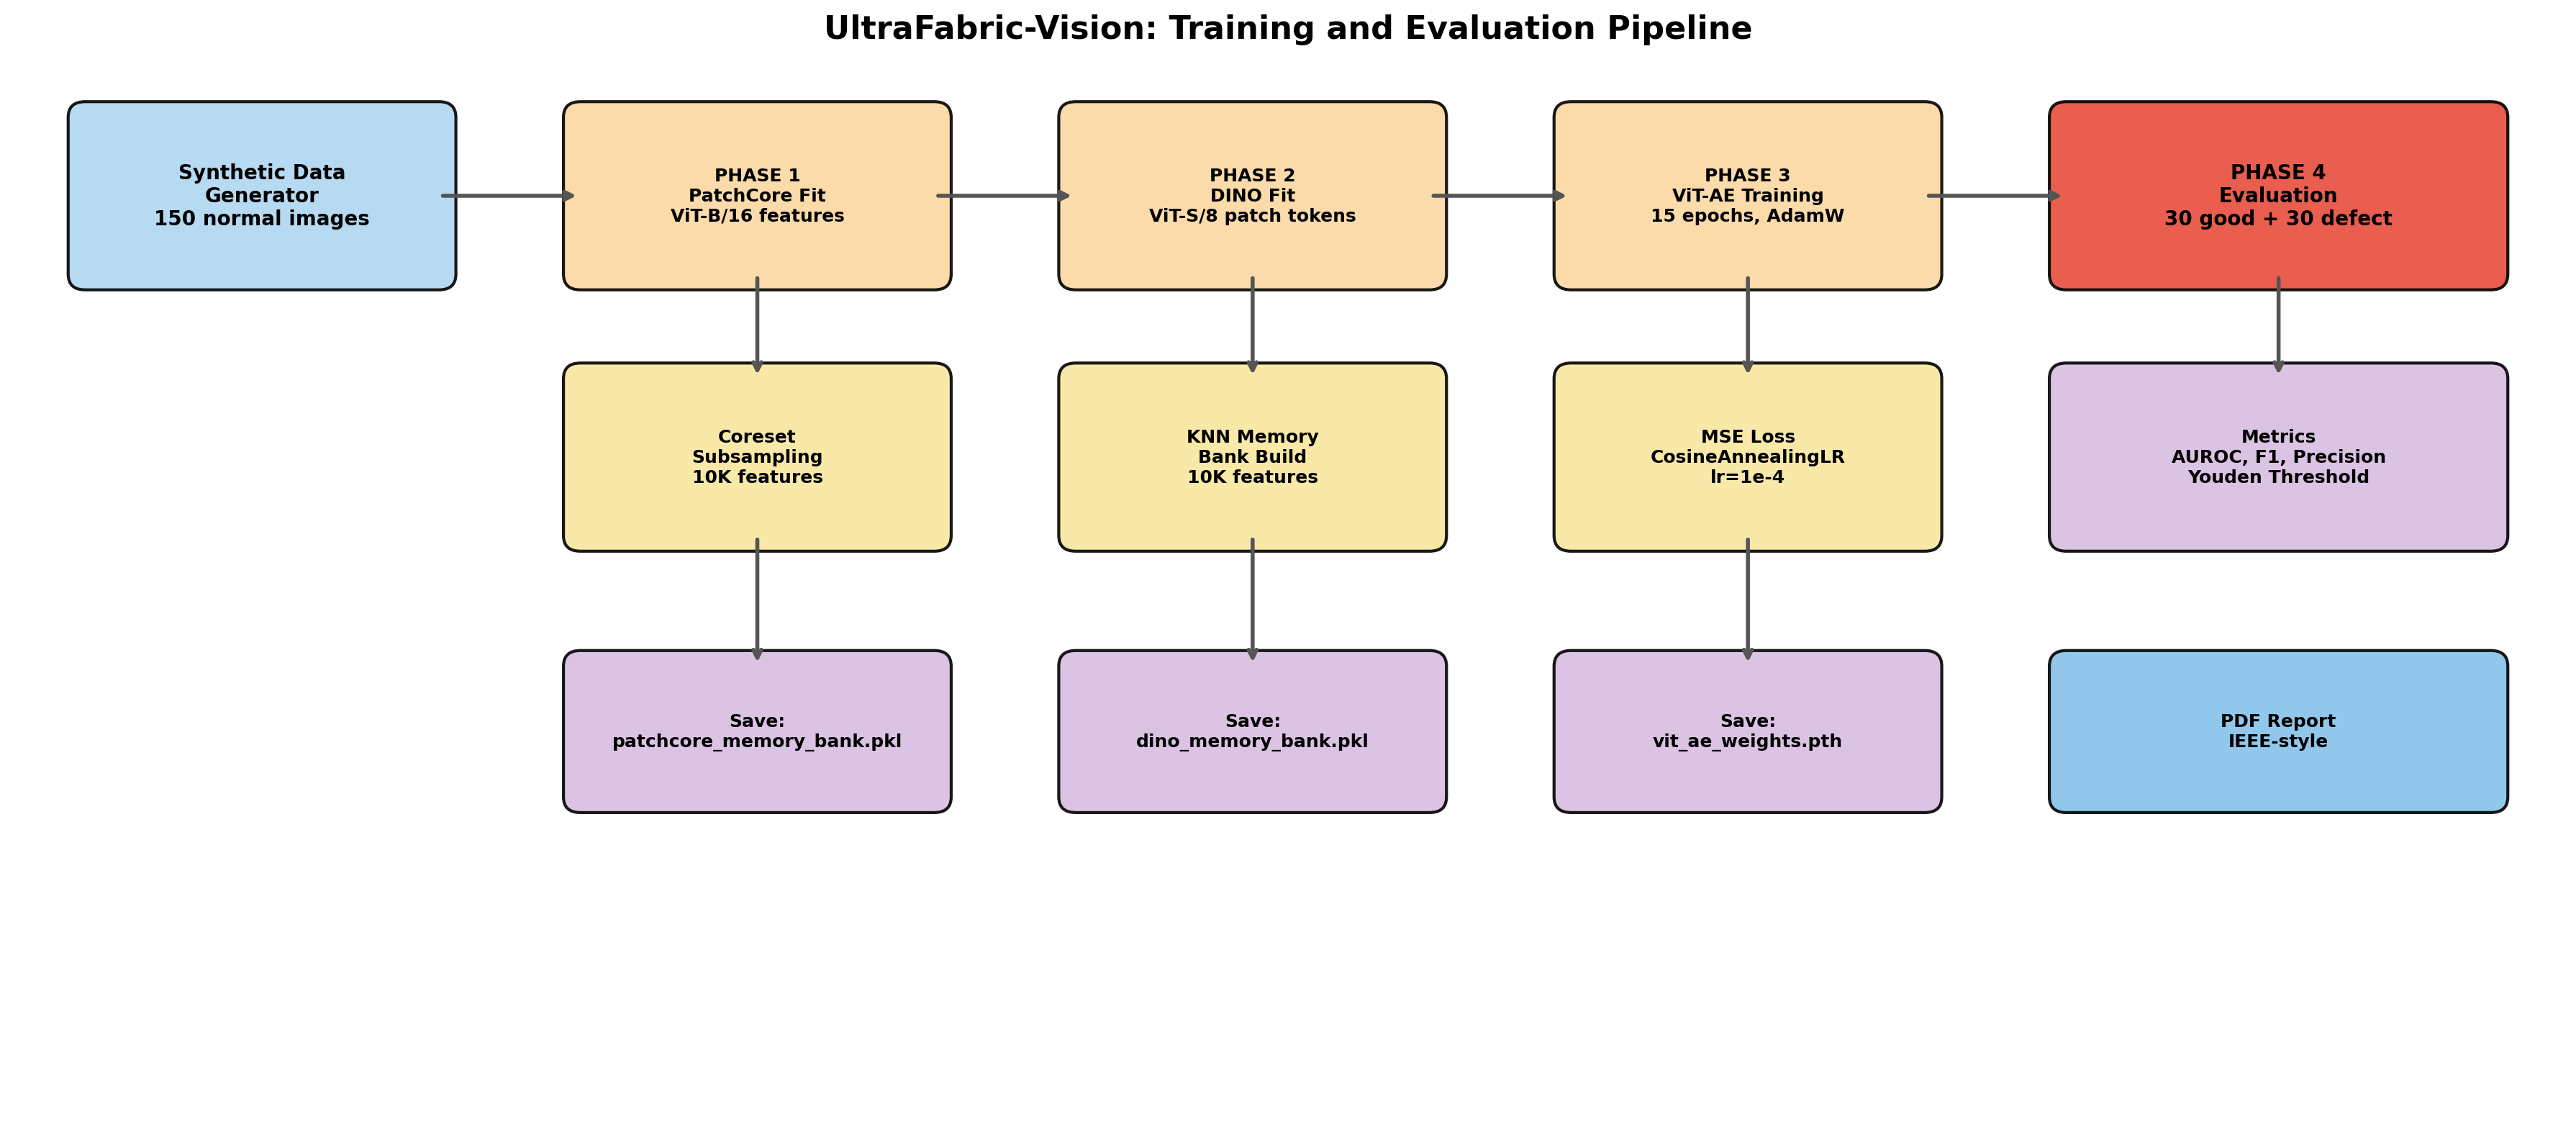
\includegraphics[width=0.95\textwidth]{Figures/training_pipeline.png}
\caption{Offline preparation pipeline: PatchCore and DINO memory-bank construction, ViT-Autoencoder training, and calibration/evaluation, producing the deployable weights and calibration artifact.}
\label{fig:pipeline}
\end{figure}

\section{Mixed Precision, Fused Attention, and Warm-up}

Three further optimizations reduce per-frame cost. The transformer backbones run under fp16 automatic mixed precision, while distance computations are kept in fp32 to preserve nearest-neighbour ordering. The DINO pathway captures its final-layer attention during the same forward pass used for scoring, avoiding a second full traversal of the network. A dummy frame is processed at start-up so that lazy CUDA initialization and kernel autotuning are paid once rather than on the first production frame.

\section{Service Stack}

The calibrated engine is exposed through three thin interfaces that share one implementation. A FastAPI application provides REST endpoints for single-image and batch inference and WebSocket endpoints for live camera streaming, with optional API-key authentication and health and version endpoints for orchestration. An embeddable \texttt{InferenceEngine} class loads the models once and scores frames directly, for integration into edge or line-control software. A batch command-line tool scores folders of images and emits CSV or JSON reports for manufacturing-execution systems. Runtime configuration is entirely environment-driven, and a GPU Docker image based on an official CUDA PyTorch runtime packages the service for deployment.

\section{Verification}

Correctness is validated by an automated end-to-end test suite exercising both the embeddable SDK and the full HTTP path---model loading, preprocessing, fusion, thresholding, and the response contract---on real good and defective samples, including malformed-input handling. All tests pass, confirming that the deployed service reproduces the calibrated decision behaviour.

\section{Operating Modes and Batch-Video Inspection}

Two operating modes are provided. \emph{Accurate} mode fuses all three detectors for maximum accuracy; \emph{Fast} mode runs the single fastest calibrated detector for latency-critical or GPU-less use. The mode is selectable per request across the SDK, CLI, REST/WebSocket API, and the dashboard.

For the industrial batch workflow, a recorded batch video is processed frame-by-frame. Assuming constant conveyor speed, the frame index maps to a physical position along the batch, so each detection is tagged with a position in metres and a segment/zone. A frame is declared defective only when the fused score exceeds the threshold and the anomaly heatmap contains a connected region that is larger than a configurable minimum area yet covers less than a maximum fraction of the frame. The minimum-area rule suppresses tiny texture speckle; the maximum-coverage rule guards against the opposite failure of distance-based detectors, in which a blank, occluded, or non-fabric frame lies far from every memory-bank vector and yields a uniformly high anomaly map---if left unchecked this paints defect boxes over the whole frame, so a frame whose anomalous area exceeds the coverage limit is treated as a non-localized whole-frame anomaly and reported as no defect rather than as heavily defective. Contiguous defective frames are merged into defect events with start/end positions, and per-zone statistics are aggregated. For each batch the system writes an annotated video, a defect-location map, and an automatically generated quality-control PDF record (verdict, defect positions, per-zone table); a batch-history view retains previously inspected batches with their pass/reject status.

In summary, the implementation turns the design into a correct, fast, and deployable system: a preprocessing fix restores accuracy, GPU-native scoring removes the latency bottleneck, calibration yields a portable decision boundary, dual operating modes and batch-video inspection support the factory workflow, and the service stack makes the model straightforward to integrate. The quantitative outcomes of these changes are reported in Chapter~5.
